% hw2.tex

% !TEX program = xelatex
%%%%%%%%%%%%%%%%%%%%
% see http://mirrors.concertpass.com/tex-archive/macros/latex/contrib/tufte-latex/sample-handout.pdf
% for how to use tufte-handout
\documentclass[a4paper, justified]{tufte-handout}

\usepackage{tikz}
\usetikzlibrary{automata, positioning, arrows}

% hw-preamble.tex

% geometry for A4 paper
% See https://tex.stackexchange.com/a/119912/23098
\geometry{
  left=20.0mm,
  top=20.0mm,
  bottom=20.0mm,
  textwidth=130mm, % main text block
  marginparsep=5.0mm, % gutter between main text block and margin notes
  marginparwidth=50.0mm % width of margin notes
}

% for colors
\usepackage{xcolor} % usage: \color{red}{text}
% predefined colors
\newcommand{\red}[1]{\textcolor{red}{#1}} % usage: \red{text}
\newcommand{\blue}[1]{\textcolor{blue}{#1}}
\newcommand{\teal}[1]{\textcolor{teal}{#1}}

\usepackage{todonotes}

% heading
\usepackage{sectsty}
\setcounter{secnumdepth}{2}
\allsectionsfont{\centering\huge\rmfamily}

% for Chinese
\usepackage{xeCJK}
\usepackage{zhnumber}
\setCJKmainfont[BoldFont=FandolSong-Bold.otf]{FandolSong-Regular.otf}

% for fonts
\usepackage{fontspec}
\newcommand{\song}{\CJKfamily{song}}
\newcommand{\kai}{\CJKfamily{kai}}

% To fix the ``MakeTextLowerCase'' bug:
% See https://github.com/Tufte-LaTeX/tufte-latex/issues/64#issuecomment-78572017
% Set up the spacing using fontspec features
\renewcommand\allcapsspacing[1]{{\addfontfeature{LetterSpace=15}#1}}
\renewcommand\smallcapsspacing[1]{{\addfontfeature{LetterSpace=10}#1}}

% for url
\usepackage{hyperref}
\hypersetup{colorlinks = true,
  linkcolor = teal,
  urlcolor  = teal,
  citecolor = blue,
  anchorcolor = blue}

\newcommand{\me}[4]{
    \author{
      {\bfseries 姓名:}\underline{#1}\hspace{2em}
      {\bfseries 学号:}\underline{#2}\hspace{2em}\\[10pt]
      {\bfseries 评分:}\underline{#3\hspace{3em}}\hspace{2em}
      {\bfseries 评阅:}\underline{#4\hspace{3em}}
  }
}

% Please ALWAYS Keep This.
\newcommand{\noplagiarism}{
  \begin{center}
    \fbox{\begin{tabular}{@{}c@{}}
      请独立完成作业,不得抄袭。\\
      若得到他人帮助, 请致谢。\\
      若参考了其它资料,请给出引用。\\
      鼓励讨论,但需独立书写解题过程。
    \end{tabular}}
  \end{center}
}

% \newcommand{\goal}[1]{
%   \begin{center}{\fcolorbox{blue}{yellow!60}{\parbox{0.50\textwidth}{\large
%     \begin{itemize}
%       \item 体会``思维的乐趣''
%       \item 初步了解递归与数学归纳法
%       \item 初步接触算法概念与问题下界概念
%     \end{itemize}}}}
%   \end{center}
% }

% Each hw consists of four parts:
\newcommand{\beginrequired}{\hspace{5em}\section{作业 (必做部分)}}
\newcommand{\beginoptional}{\section{作业 (选做部分)}}
\newcommand{\beginot}{\section{Open Topics}}
\newcommand{\begincorrection}{\section{订正}}
\newcommand{\beginfb}{\section{反馈}}

% for math
\usepackage{amsmath, mathtools, amsfonts, amssymb}
\newcommand{\set}[1]{\{#1\}}

% define theorem-like environments
\usepackage[amsmath, thmmarks]{ntheorem}

\theoremstyle{break}
\theorempreskip{2.0\topsep}
\theorembodyfont{\song}
\theoremseparator{}
\newtheorem{problem}{题目}[subsection]
\renewcommand{\theproblem}{\arabic{problem}}
\newtheorem{ot}{Open Topics}

\theorempreskip{3.0\topsep}
\theoremheaderfont{\kai\bfseries}
\theoremseparator{:}
\theorempostwork{\bigskip\hrule}
\newtheorem*{solution}{解答}
\theorempostwork{\bigskip\hrule}
\newtheorem*{revision}{订正}

\theoremstyle{plain}
\newtheorem*{cause}{错因分析}
\newtheorem*{remark}{注}

\theoremstyle{break}
\theorempostwork{\bigskip\hrule}
\theoremsymbol{\ensuremath{\Box}}
\newtheorem*{proof}{证明}

% \newcommand{\ot}{\blue{\bf [OT]}}

% for figs
\renewcommand\figurename{图}
\renewcommand\tablename{表}

% for fig without caption: #1: width/size; #2: fig file
\newcommand{\fig}[2]{
  \begin{figure}[htbp]
    \centering
    \includegraphics[#1]{#2}
  \end{figure}
}
% for fig with caption: #1: width/size; #2: fig file; #3: caption
\newcommand{\figcap}[3]{
  \begin{figure}[htbp]
    \centering
    \includegraphics[#1]{#2}
    \caption{#3}
  \end{figure}
}
% for fig with both caption and label: #1: width/size; #2: fig file; #3: caption; #4: label
\newcommand{\figcaplbl}[4]{
  \begin{figure}[htbp]
    \centering
    \includegraphics[#1]{#2}
    \caption{#3}
    \label{#4}
  \end{figure}
}
% for margin fig without caption: #1: width/size; #2: fig file
\newcommand{\mfig}[2]{
  \begin{marginfigure}
    \centering
    \includegraphics[#1]{#2}
  \end{marginfigure}
}
% for margin fig with caption: #1: width/size; #2: fig file; #3: caption
\newcommand{\mfigcap}[3]{
  \begin{marginfigure}
    \centering
    \includegraphics[#1]{#2}
    \caption{#3}
  \end{marginfigure}
}

\usepackage{fancyvrb}

% for algorithms
\usepackage[]{algorithm}
\usepackage[]{algpseudocode} % noend
% See [Adjust the indentation whithin the algorithmicx-package when a line is broken](https://tex.stackexchange.com/a/68540/23098)
\newcommand{\algparbox}[1]{\parbox[t]{\dimexpr\linewidth-\algorithmicindent}{#1\strut}}
\newcommand{\hStatex}[0]{\vspace{5pt}}
\makeatletter
\newlength{\trianglerightwidth}
\settowidth{\trianglerightwidth}{$\triangleright$~}
\algnewcommand{\LineComment}[1]{\Statex \hskip\ALG@thistlm \(\triangleright\) #1}
\algnewcommand{\LineCommentCont}[1]{\Statex \hskip\ALG@thistlm%
  \parbox[t]{\dimexpr\linewidth-\ALG@thistlm}{\hangindent=\trianglerightwidth \hangafter=1 \strut$\triangleright$ #1\strut}}
\makeatother

% for footnote/marginnote
% see https://tex.stackexchange.com/a/133265/23098
\usepackage{tikz}
\newcommand{\circled}[1]{%
  \tikz[baseline=(char.base)]
  \node [draw, circle, inner sep = 0.5pt, font = \tiny, minimum size = 8pt] (char) {#1};
}
\renewcommand\thefootnote{\protect\circled{\arabic{footnote}}}

\newcommand{\score}[1]{{\bf [#1 分]}}

\newcommand{\rel}[1]{\xrightarrow{#1}}
\newcommand{\dstar}{\xRightarrow[]{\ast}}
\newcommand{\dplus}{\xRightarrow[]{+}}
\newcommand{\lm}{\xRightarrow[\text{lm}]{}}
\renewcommand{\rm}{\xRightarrow[\text{rm}]{}}
\newcommand{\dpluslm}{\xRightarrow[\text{lm}]{+}}
\newcommand{\dstarlm}{\xRightarrow[\text{lm}]{\ast}}
\newcommand{\dplusrm}{\xRightarrow[\text{rm}]{+}}
\newcommand{\dstarrm}{\xRightarrow[\text{rm}]{\ast}}

\newcommand{\forkw}{\text{\bf for}}
\newcommand{\ifkw}{\text{\bf if}}
\newcommand{\printkw}{\text{\bf print}}

\newcommand{\first}{\textsc{First}}
\newcommand{\follow}{\textsc{Follow}}

% see https://tex.stackexchange.com/a/109906/23098
\usepackage{empheq}
\newcommand*\widefbox[1]{\fbox{\hspace{2em}#1\hspace{2em}}} % feel free to modify this file if you understand LaTeX well
%%%%%%%%%%%%%%%%%%%%
\title{编译原理作业 (2)}
\me{\hspace{50pt}}{\hspace{70pt}}{}{}
\date{2022年11月16日}
%%%%%%%%%%%%%%%%%%%%
\begin{document}
\maketitle
%%%%%%%%%%%%%%%%%%%%
\noplagiarism % PLEASE DON'T DELETE THIS LINE!
%%%%%%%%%%%%%%%%%%%%
\begin{abstract}
\end{abstract}
%%%%%%%%%%%%%%%%%%%%
\beginrequired
%%%%%%%%%%%%%%%

%%%%%%%%%%%%%%%
\begin{problem}[正则表达式与自动机]
  考虑正则表达式 $r = (1 \mid 01)^{\ast} 0^{\ast}$ (字母表 $\Sigma = \set{0, 1}$)。
  \sidenote{
    如何用 \LaTeX{} 写(复杂的)正则表达式?
    \begin{itemize}
      \item \href{https://tex.stackexchange.com/a/162122/23098}{How to escape properly and output regex in latex?@tex.stackexchange}
    \end{itemize}
    如何用 \LaTeX{} 画自动机?
    \begin{itemize}
      \item \href{https://www3.nd.edu/~kogge/courses/cse30151-fa17/Public/other/tikz\_tutorial.pdf}{使用{\texttt{tikz automata}} library}
      \item \href{https://hayesall.com/blog/latex-automata/}{另一个关于\texttt{tikz automata}的教程}
      \item 在 \href{https://notendur.hi.is/aee11/automataLatexGen/}{网站\texttt{automataLatexGen}生成\LaTeX{}代码}
      \item \red{使用 \href{https://www.jflap.org/}{\texttt{jflap}} 工具 ({\bf 推荐学习该工具})}
    \end{itemize}
  }
  \begin{enumerate}[(1)]
    \item 使用 Thompson 构造法构造等价的 NFA;
    \item 使用子集构造法构造等价的 DFA;
    \item 将上一步构造的 DFA 最小化;
  \end{enumerate}
  以上各小题, 请给出关键的中间步骤。

  \noindent (不必给出所有的细节, 类似的步骤可以``跳步'')
\end{problem}

\begin{solution}
	 (1)\\
	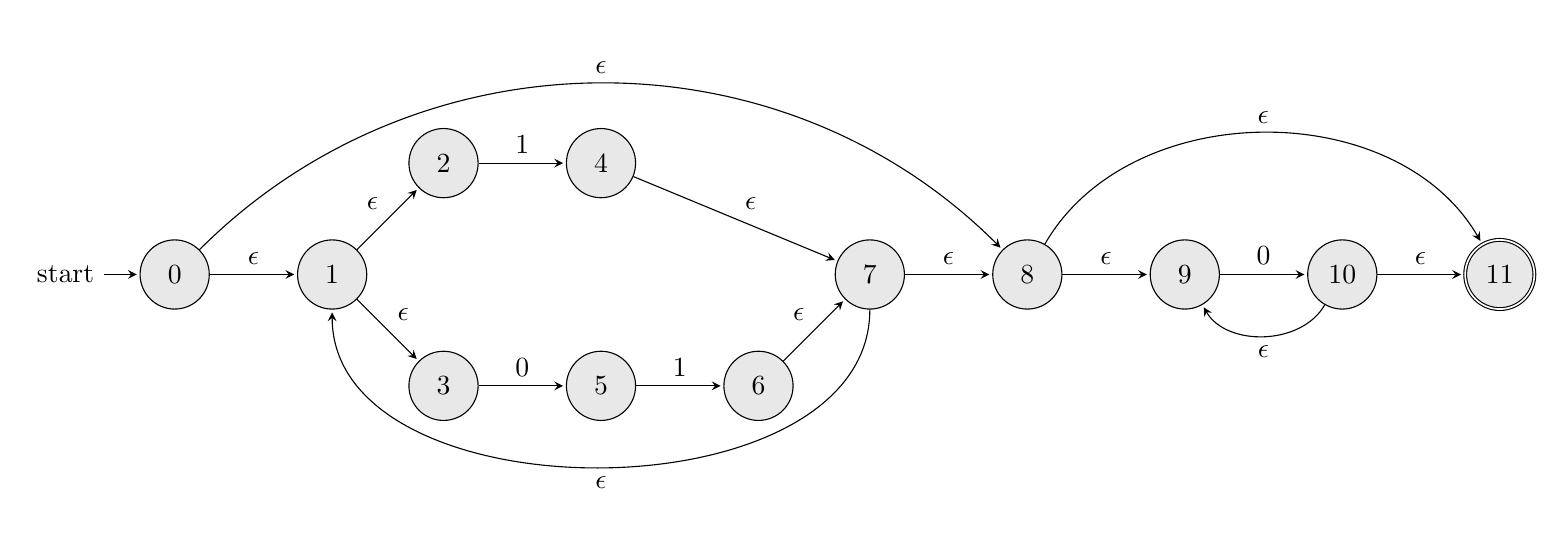
\begin{tikzpicture}[->,>=stealth,shorten >=1pt,auto,node distance=2cm,
		scale = 1,transform shape]
		\tikzstyle{every state}=[fill={rgb:black,1;white,10}]
		\node[state] (0) [initial]{$0$};
		\node[state] (1) [right of=0] {$1$};
		\node[state] (2) [above right of=1] {$2$};
		\node[state] (3) [below right of=1] {$3$};
		\node[state] (4) [right of=2] {$4$};
		\node[state] (5) [right of=3] {$5$};
		\node[state] (6) [right of=5] {$6$};
		\node[state] (7) [above right of=6] {$7$};
		\node[state] (8) [right of=7] {$8$};
		\node[state] (9) [right of=8] {$9$};
		\node[state] (10) [right of=9] {$10$};
		\node[state, accepting] (11) [right of=10] {$11$};

		\path 	(0)  edge			   node {$\epsilon$} (1)
				(0)  edge[bend left=45]node {$\epsilon$} (8)
				(1)  edge              node {$\epsilon$} (2)
				(1)  edge              node {$\epsilon$} (3)
				(2)  edge              node {$1$} (4)
				(3)  edge              node {$0$} (5)
				(4)  edge              node {$\epsilon$} (7)
				(5)  edge              node {$1$} (6)
				(6)  edge              node {$\epsilon$} (7)
				(7)  edge              node {$\epsilon$} (8)
				(7)  edge[bend left=90]node {$\epsilon$} (1)
				(8)  edge              node {$\epsilon$} (9)
				(8)  edge[bend left=60]node {$\epsilon$} (11)
				(9)  edge              node {$0$} (10)
				(10) edge[bend left=60]node {$\epsilon$} (9)
				(10) edge              node {$\epsilon$} (11);
	\end{tikzpicture}
\\
(2)\\
\begin{table}[ht]
	\begin{tabular}{|l|l|l|l|l|}
		\hline
		\textbf{NFA状态} 		& \textbf{DFA状态} & \textbf{0} & \textbf{1}	  \\ \hline
		{0,1,2,3,8,9,11}      & A               & B          & C          	 \\ \hline
		{5,9,10,11}           & B               & D          & E             \\ \hline
		{1,2,3,4,7,8,9,11}    & C               & B          & C     		 \\ \hline
		{9,10,11}             & D               & D          & $\varnothing$ \\ \hline
		{1,2,3,6,7,8,9,11}    & E               & B			 & C     		 \\ \hline
	\end{tabular}
\end{table}
\\
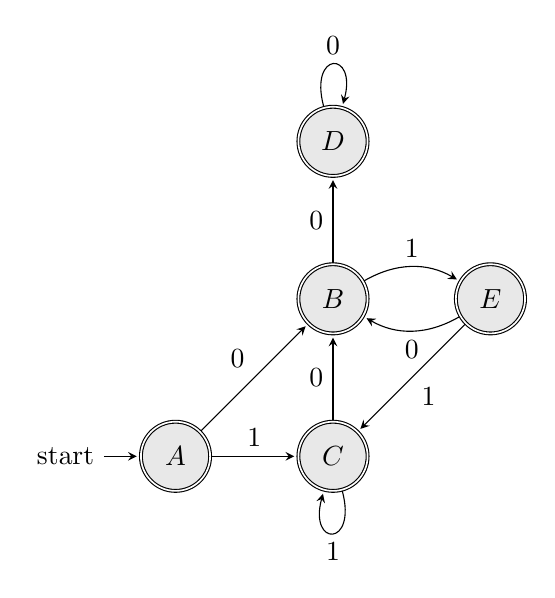
\begin{tikzpicture}[->,>=stealth,shorten >=1pt,auto,node distance=2cm,
	scale = 1,transform shape]
	\tikzstyle{every state}=[fill={rgb:black,1;white,10}]
	\node[state,accepting] (A) [initial] {$A$};
	\node[state,accepting] (C) [right of=A] {$C$};
	\node[state,accepting] (B) [above of=C] {$B$};
	\node[state,accepting] (D) [above of=B] {$D$};
	\node[state,accepting] (E) [right of=B] {$E$};
	
	\path 	
		(A)  edge              node {$0$} (B)
		(A)  edge			   node {$1$} (C)
		(B)  edge              node {$0$} (D)
		(B)  edge[bend left=30]node {$1$} (E)
		(C)  edge[loop below]  node {$1$} (C)
		(C)  edge              node {$0$} (B)
		(D)  edge[loop above]  node {$0$} (D)
		(E)  edge[bend left=30]node {$0$} (B)
		(E)  edge              node {$1$} (C);
\end{tikzpicture} 
\\
(3)\\
$\Pi_{0}=\{\{A,B,C,D,E\}\}$\\
$\Pi_{1}=\{\{A,B,C,E\},\{D\}\}\}$\\
$\Pi_{2}=\{\{A,C,E\},\{B\},\{D\}\}\}$\\
$\Pi_{3}=\Pi_{2}=\Pi_{final}$\\
或者可以直接看出来合并A,C,E\\
$a=\{A,C,E\}$\\
$b=\{B\}$\\
$c=\{D\}$\\
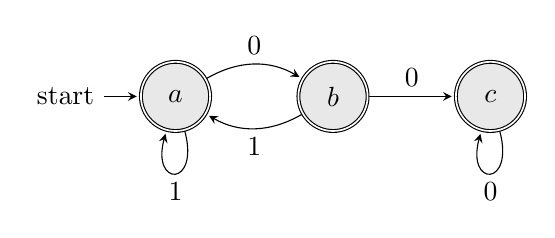
\begin{tikzpicture}[->,>=stealth,shorten >=1pt,auto,node distance=2cm,
	scale = 1,transform shape]
	\tikzstyle{every state}=[fill={rgb:black,1;white,10}]
	\node[state,accepting] (a) [initial] {$a$};
	\node[state,accepting] (b) [right of=a] {$b$};
	\node[state,accepting] (c) [right of=b] {$c$};
	\path 	
	(a)  edge[loop below]  node {$1$} (a)
	(a)  edge[bend left=30]node {$0$} (b)
	(b)  edge[bend left=30]node {$1$} (a)
	(b)  edge 			   node {$0$} (c)
	(c)  edge[loop below]  node {$0$} (c);
\end{tikzpicture} 
\end{solution}
%%%%%%%%%%%%%%%

%%%%%%%%%%%%%%%%%%%%
% 如果没有需要订正的题目,可以把这部分删掉

% \begincorrection
%%%%%%%%%%%%%%%%%%%%

%%%%%%%%%%%%%%%%%%%%
% 如果没有反馈,可以把这部分删掉
\beginfb

你可以写 (若无内容, 可删除该节)
\begin{itemize}
  \item 对课程及教师的建议与意见
  \item 教材中不理解的内容
  \item 希望深入了解的内容
  \item $\cdots$
\end{itemize}
%%%%%%%%%%%%%%%%%%%%
\end{document}